% Template last modified by Jake Hart; please contact course staff if you have any questions regarding using this template

\documentclass{cisXXX} % You must have the cisXXX .cls file in your project or working directory (i.e. the same directory as this document) 

\HWauthor{Zeyu Zhao}{zhaozeyu@seas.upenn.edu} % Put your name and Penn email on this line
\HWno{11} % Enter the number of the homework you are working on
\HWcourse{ESE 303} % Enter the course department and number here
%\HWpartner{Paul Brown} % If your class allows group work, put your partners here
%\HWpartner{Amelia Earhart} % Otherwise, delete or comment these lines 
\usepackage{amsmath}
\usepackage{amsfonts}
% code
\usepackage{color}
\usepackage[framed,numbered,autolinebreaks,useliterate]{mcode}
\usepackage{graphicx}
\definecolor{dkgreen}{rgb}{0,0.6,0}
\definecolor{gray}{rgb}{0.5,0.5,0.5}
\definecolor{mauve}{rgb}{0.58,0,0.82}
\begin{document}
\maketitle
\HWproblem
From the definition of WGN $W(t)$ and the property (1) of Gaussian process we know that $W \left( t _ { 1 } \right)$ and $W \left( t _ { 2 } \right)$ are jointly Gaussian. Jointly normal random variables are independent if and only if the correlation between $W \left( t _ { 1 } \right)$ and $W \left( t _ { 2 } \right)$ is 0. Therefore, it suffices to show that $W \left( t _ { 1 } \right)$ and $W \left( t _ { 2 } \right)$ are not correlated, for $t _ { 1 } \neq t _ { 2 }$.  
	This is true because the autocorrection function $R _ { W } \left( t _ { 1 } , t _ { 2 } \right) = 0$ for $t _ { 1 } \neq t _ { 2 }$. The reason is that the Dirac delta function $\delta(t) = 0, \forall t \neq 0$.
\HWproblem
$X ( t )$ is a Gaussian process since it is an integration of Gaussian processes, and because a linear functional of Gaussian processes is still a Gaussian process (property 1 of Gaussian processes).

The mean of $X ( t )$:

$$
\mu _ { X } ( t ) = \mathbb { E } \left[ \int _ { 0 } ^ { t } W ( 
\tau ) d \tau \right] = \int _ { 0 } ^ { t } \mathbb { E } [ W ( \tau ) ] d \tau = \int _ { 0 } ^ { t } \mu _ { W } ( \tau ) d \tau = 0
$$
The reason is that $\delta ( \tau ) = 0$ for $\tau \neq 0$.

The autocorrelation function of $X ( t )$:
$$
\begin{aligned} R _ { X } \left( t _ { 1 } , t _ { 2 } \right) & = \mathbb { E } \left[ \left( \int _ { 0 } ^ { t _ { 1 } } W \left( \tau _ { 1 } \right) d \tau _ { 1 } \right) \left( \int _ { 0 } ^ { t _ { 2 } } W \left( \tau _ { 2 } \right) d \tau _ { 2 } \right) \right] \\ & = \mathbb { E } \left[ \int _ { 0 } ^ { t _ { 1 } } \int _ { 0 } ^ { t _ { 2 } } W \left( \tau _ { 1 } \right) W \left( \tau _ { 2 } \right) d \tau _ { 2 } d \tau _ { 1 } \right] \\ & = \int _ { 0 } ^ { t _ { 1 } } \int _ { 0 } ^ { t _ { 2 } } \mathbb { E } \left[ W \left( \tau _ { 1 } \right) W \left( \tau _ { 2 } \right) \right] d \tau _ { 2 } d \tau _ { 1 } \\ & = \int _ { 0 } ^ { t _ { 1 } } \int _ { 0 } ^ { t _ { 2 } } R _ { W } \left( \tau _ { 1 } , \tau _ { 2 } \right) d \tau _ { 2 } d \tau _ { 1 } \\ & = \int _ { 0 } ^ { t _ { 1 } } \int _ { 0 } ^ { t _ { 2 } } \sigma ^2 \delta \left( \tau _ { 1 } - \tau _ { 2 } \right) d \tau _ { 2 } d \tau _ { 1 } \end{aligned}
$$
Now, from the properties of Dirac delta function and what we learned in class:
\begin{align*}
R _ { X } \left( t _ { 1 } , t _ { 2 } \right) &= \left\{ \begin{array} { l l } { \int _ { 0 } ^ { t _ { 1 } } \sigma ^ { 2 } d \tau _ { 1 } = \sigma ^ { 2 } t _ { 1 } , } & { \text { for } t _ { 1 } < t _ { 2 } } \\ { \int _ { 0 } ^ { t _ { 2 } } \sigma ^ { 2 } d \tau _ { 2 } = \sigma ^ { 2 } t _ { 2 } , } & { \text { for } t _ { 1 } > t _ { 2 } } \end{array} \right. \\ 
&= \sigma ^ { 2 } \min \left( t _ { 1 } , t _ { 2 } \right)
\end{align*}
Therefore, the gaussian process at time $t$ is a normal distribution $X ( t ) \sim \mathcal { N } \left( \mu_X ( t ) , \sqrt { R _ { X } ( t , t ) } \right) = \mathcal { N } \left( 0, \sigma \sqrt {t} \right)$. Hence,
$$
\mathbb { P } [ X ( t ) > a ] = 1 - \mathbb { P } [ X ( t ) \leq a ] = 1 - \Phi \left( \frac { a } { \sigma \sqrt { t } } \right)
$$
where $\Phi$ is the cdf of the standard Gaussian.

\HWproblem
Similar to Problem 2, $W _ { h } ( n )$ is still a Gaussian Process since integration is linear functional.
The mean of  $W _ { h } ( n )$:
$$
\mu _ { W _ { h } } ( n ) = \mathbb { E } \left[ W _ { h } ( n ) \right] = \mathbb { E } \left[ \int _ { n h } ^ { ( n + 1 ) h } W ( \tau ) d \tau \right] = \int _ { n h } ^ { ( n + 1 ) h } \mathbb { E } [ W ( \tau ) ] d \tau = \int _ { n h } ^ { ( n + 1 ) h } 0 d \tau = 0
$$
The autocorrelation function of  $W _ { h } ( n )$:

$$\begin{aligned} 
	R _ { W _ { h } } \left( n _ { 1 } , n _ { 2 } \right) & = \mathbb { E } \left[ W _ { h } \left( n _ { 1 } \right) W _ { h } \left( n _ { 2 } \right) \right] \\ 
	& = \mathbb { E } \left[ \left( \int _ { n _ { 1 } h } ^ { \left( n _ { 1 } + 1 \right) h } W \left( \tau _ { 1 } \right) d \tau _ { 1 } \right) \left( \int _ { n _ { 2 } h } ^ { \left( n _ { 2 } + 1 \right) h } W \left( \tau _ { 2 } \right) d \tau _ { 2 } \right) \right] \\ 
	& = \mathbb { E } \left[ \int _ { n _ { 1 } h } ^ { \left( n _ { 1 } + 1 \right) h } \int _ { n _ { 2 } h } ^ { \left( n _ { 2 } + 1 \right) h } W \left( \tau _ { 1 } \right) W \left( \tau _ { 2 } \right)  d \tau _ { 2 } d \tau _ { 1 } \right] \\ 
	& = \int _ { n _ { 1 } h } ^ { \left( n _ { 1 } + 1 \right) h } \int _ { n _ { 2 } h } ^ { \left( n _ { 2 } + 1 \right) h } \sigma^2 \delta \left( \tau _ { 1 } - \tau _ { 2 } \right) d \tau _ { 2 } d \tau _ { 1 }  \\ 
	& = \left\{ \begin{array} { l } { 0 , \quad n _ { 1 } \neq n _ { 2 }  } \\ { \sigma ^ { 2 } h , \quad n _ { 1 } = n _ { 2 }} \end{array} \right. 
\end{aligned}$$

\HWproblem
The following MATLAB script simulates the process $X(t)$  using its discrete time version $X_h(n)$ obtained from $W_h(n)$ derived in Part C.
\lstinputlisting{D_code.m}
A result of this simulation is shown in Figure \ref{fig:D1}.
\begin{figure}
  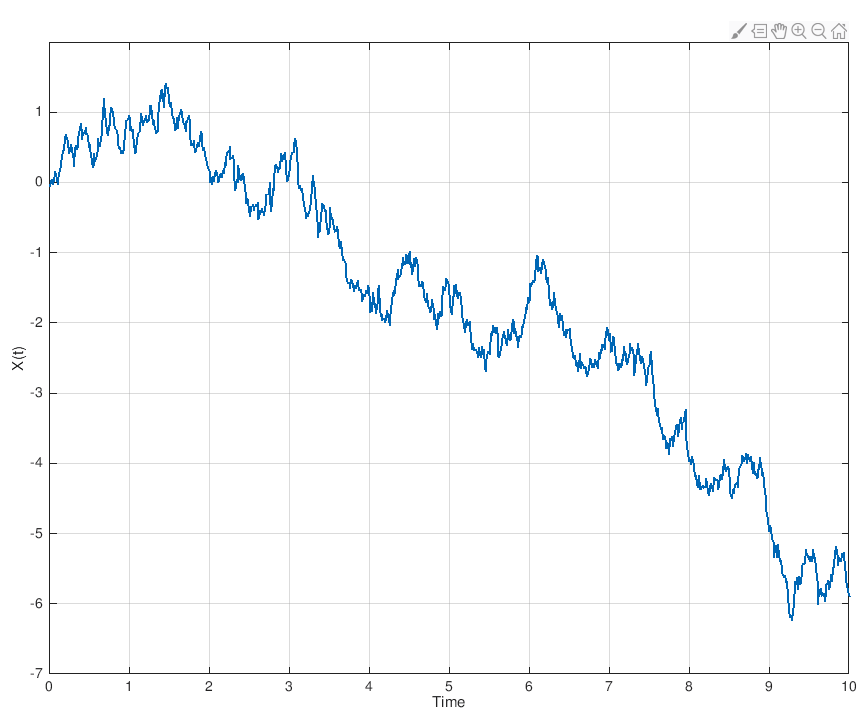
\includegraphics[width=\linewidth]{D_plot.png}
  \caption{A sample path of the simulated Gaussian (Wiener) process $X(t)$ using a discrete approximation
with step size $h = 0.01$ (part D).}
  \label{fig:D1}
\end{figure}

\end{document}